\section{Variational Autoencoders}

  Note that like linear latent variable models such as PCA, autoencoders ``encode'' our samples in a latent space, which we will call $\mathcal{Z}$. If we wanted to create a generative model from autoencoders, we can use the analogous transition from PCA to PPCA, by changing our points to distributions. Like in PPCA, we might want to define a standard Gaussian over the latent space $\mathcal{Z}$ and transform this into the original space $\mathcal{X}$. However, there is a small problem with autoencoders. The latent space where the encoded vectors lie may not be contiguous, which means that the distribution of the latent space may not be very simple either. Look at the encodings of MNIST below. Trying to sample from this space with a isotropic Gaussian results in a high probability of hitting the ``dead'' zones which may give garbage generative results. If the space has discontinuities and you sample a variation from there, the decoder will simply generate an unrealistic output. 

  \begin{figure}[H]
    \centering
    \begin{subfigure}[b]{0.48\textwidth}
      \centering
      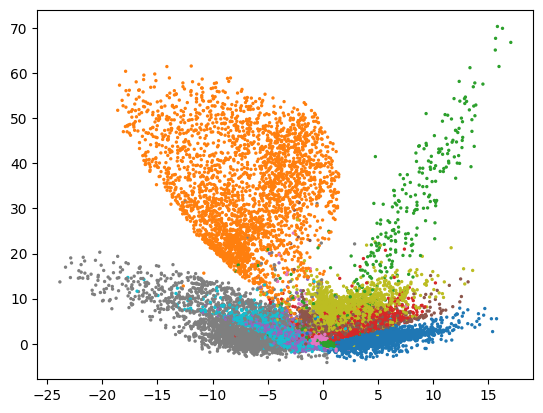
\includegraphics[scale=0.36]{img/08_VAE/mnist_latent.png}
      \caption{Training an autoencoder on MNIST and then visualizing the encodings from a 2D latent space shows the formation of distinct clusters, but there are huge empty spaces where the labeling may be ambiguous and not allow us to interpolate effectively. }
      \label{fig:mnist_latent}
    \end{subfigure}
    \hfill 
    \begin{subfigure}[b]{0.48\textwidth}
      \centering
      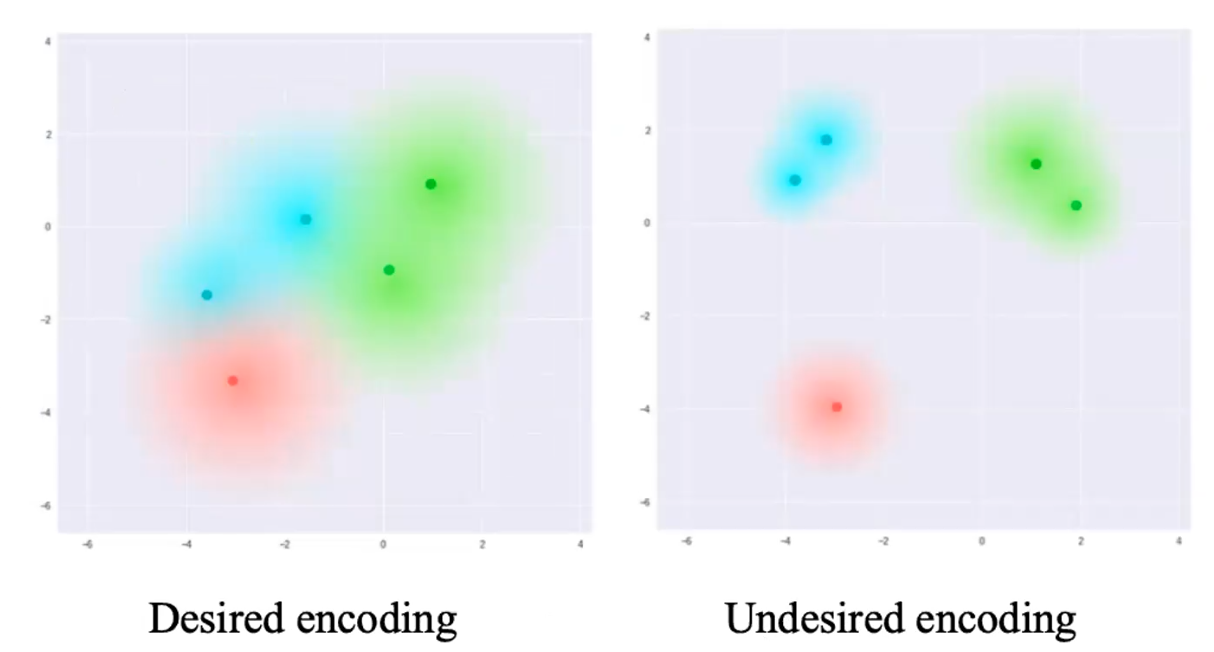
\includegraphics[scale=0.22]{img/08_VAE/contiguous_encoding.png}
      \caption{ Therefore, we want the encodings to be contiguous while still being distinct. This allows smooth interpolation which is easy to sample from with a simple pdf, e.g. Gaussian, and enables construction of \textit{new} samples. } 
      \label{fig:contiguous_encoding}
    \end{subfigure}
    \caption{}
    \label{fig:motivation_vae}
  \end{figure}

  In 2013, Kigma introduced this generative model that bridges between latent variable models and deep neural nets. We can think of the relationship between the linear model PCA and its latent counterpart PPCA as the relationship between the nonlinear autoencoders and variational autoencoders. This is a good time to review linear and nonlinear latent variable models in my ML notes. Note that in a LVM, the family of functions $\{D_\beta\}$ is used to map a latent variable $z$ to the likelihood $p(x \mid z)$. This can be done by a direct transformation of the random variable $Z$ (e.g. PPCA or as we will see later, \textit{normalizing flows}), or we can have $D_\beta(z)$ be an explicit parameterization (e.g. Gaussian mixture models and variational autoencoders). Given neural networks, we can do the latter method quite easily, and we are already familiar with the architectures to do so. 

  \begin{example}[Classification Nets Parameterize Multinomials]
    In a classification neural network with parameters $\beta$, it takes in an input $x$ and outputs a softmax vector $f_\beta (x) =(p_1, \ldots, p_K)^T$. This basically means that $f_\beta (x) = \theta$ parameterizes the conditional distribution (in this case, multinomial) of $y$ given $x$. 
    \begin{equation}
      Y \mid X = x \sim \mathrm{Multinomial}(\theta = f_\beta (x))
    \end{equation}
    This is a much more efficient way to store conditional distributions than a $\dim(X) (K - 1)$ lookup table. 
  \end{example}

  Therefore, by generating a latent variable $p(z)$ (that is simple and fixed), we can use a deep neural network $D_\beta$ to generate $\theta = D_\beta (z)$ which serve as the parameters of the conditional distribution $p_\theta (x \mid z)$, and then sampling from this distribution is easy because we assume that $p_\theta (x \mid z)$ is in an explicitly parameterized family of distributions. This allows us to easily sample from the joint distribution. 
  \begin{equation}
    p_\theta (x, z) = p_\theta (x \mid z) \, p(z)
  \end{equation}
  This is all great, but computing 
  \begin{equation}
    p(x) = \int p(x, z) \,dz = \int p_\theta (x \mid z) \, p(z) \,dz
  \end{equation}
  is computationally intractable. With strong assumptions, like conditional independence of not just $p(x \mid z)$ but \textit{also} $p(z \mid x)$, in RBMs, we can construct pretty good approximations. Recall that for RBMs, the derivative of the log of $p(x)$ decomposes into a positive phase that requires you to integrate over $p(z \mid x)$, which is easy, and $p(x, h)$, which is hard to do in general. But through contrastive divergence, we can approximate the integral by sampling a $\Tilde{x}$ and constructing another integral over $p(z \mid x)$, which is then easy to compute. 

  \begin{example}[Bernoulli-Bernoulli RBM] 
    We would like to approximate a $d$-dimensional Bernoulli vector $x$ with a latent variable $z \in \mathbb{R}^K$. We will assume a prior $p(z) \sim N(0, I)$, and let us have a neural net $D_{\beta}$ that parameterizes the random vector $x$, where $x_i \sim \mathrm{Bernoulli}(\theta_i)$ for $\theta_i$. Then, by conditional independence, 
    \begin{equation}
      p(x \mid z) = \prod_{i=1}^d p_\theta (x_i \mid z) = \prod_{i=1}^d \theta_i^{x_i} (1 - \theta_i)^{1 - x_i} = \prod_{i=1}^d \big[ D_\beta(z) \big]_i^{x_i} \big( 1 - [D_\beta(z)]_d \big)^{1 - x_i}
    \end{equation}
    and we can see that since $p$ has the flexibility of whatever vector in $[0, 1]^D$ it can be captured by the neural net $D_\beta$. It encompasses a broad family of Bernoulli probability distributions. We can see that we have some method to compute $p(x \mid z)$. We train a neural net (somehow) and do forward prop on it to generate the correct parameters modeling the distribution of $x$. Note that in RBMs the conditional independence allowed us to integrate over $z$ easily. To see why, in the example above, the integral becomes
    \begin{equation}
      p(x) = \sum_{z \in \{0, 1\}^k} \bigg\{ \prod_{i=1}^d \big[ D_\beta(z) \big]_i^{x_i} \big( 1 - [D_\beta(z)]_d \big)^{1 - x_i} \bigg\} p(z) 
    \end{equation}
    where $k$ is the dimension of the latent space. However, integrating over all $z$'s for more complex spaces is not feasible. 
  \end{example}

  $D_\beta$ is clearly nonlinear and we can't just do some simple closed form optimization, so we must use the tools introduced in nonlinear latent variable models. Namely, we revisit the variational lower bound. Recall that estimating the true $p(x)$ can be reduced to the problem of finding a good approximate of the true $p(z \mid x)$, the \textit{posterior} or \textit{inference component}, with some family of distributions $\{ q_\phi \}$. Just like the generation model, we can build another neural network $E_{\alpha}$ such that $\phi = E_{\alpha} (x)$ parameterizes the conditional distribution of $z$, called our \textit{encoder}. 
  \begin{equation}
    p(z \mid x) \approx q_\phi (z \mid x) = q_{E_\alpha (x)} (z)
  \end{equation}

  \begin{example}[Encoder Neural Net Generates Parameters of Likelihood]
    If $\phi = (\mu, \sigma)$, where $\sigma$ is just the vector representing variances of independent Gaussians, then we can use the neural network $E$ to get $\phi = E_{\alpha} (x)$. In the example, $\phi = (\mu, \log \sigma^2)$ since we want to allow negative values, and 
    \begin{equation}
      q_\phi (z \mid x) \sim \mathcal{N}(E_\alpha (x)) = \mathcal{N}(\phi) = \mathcal{N} (\mu, \sigma^2)
    \end{equation}
  \end{example} 

  Therefore, by modeling both the likelihood and posterior with probability distributions that can be parameterized by an output of neural networks, we have a \textit{variational autoencoder}. 

  \begin{definition}[Variational Autoencoders]
    In a \textbf{variational autoencoder (VAE)}, we assume that the covariates $x^{(i)} \sim X$ are generated as the marginal of a joint distribution $p(x, z)$ with latent variable $z \sim X$. We model the sub-distributions as such: 
    \begin{enumerate}
      \item We assume that the prior $p(z)$ is of fixed simple form, e.g. a standard Gaussian. 
      \item We assume that the likelihood $p(x \mid z)$ can be approximated by a parameteric family of distributions $p_\theta (x \mid z)$, where $\theta = D_\beta (z)$ is generated by a \textbf{decoder} neural network parameterized by $\beta$.
      \item We assume that the posterior $p(z \mid x)$ can be approximated by a parameteric family of distributions $q_\phi (z \mid x)$,\footnote{Note that this is an assumption! The posterior may be an arbitrary shape or form.} where $\phi = E_\alpha (x)$ is generated by an \textbf{encoder} neural network parameterized by $\alpha$.
    \end{enumerate} 
    We can optimize $\theta, \lambda$ by equivalently optimizing the parameters $\alpha, \beta$ of the nets. Once this is done, 
    \begin{enumerate}
      \item To conduct inference, we can input in some data $x$ and retrieve the distribution of its latent representation as $q_{E_\alpha (x)} \approx p (z \mid x)$. 
      \item To generate data, we can sample $z$ from $p(z)$ and sample from $p_{D_\beta (z)} (x) \approx p (x \mid z)$. 
    \end{enumerate}
  \end{definition} 

  So how do we actually train this? Just like with every other nonlinear latent variable models, we can use the evidence lower bound. We do a quick review. Recall that the KL divergence can be decomposed into the sum of conditional entropies, and hence we can use the fact the KL divergence is always nonnegative to create this bound. 
  \begin{align}
    \log p_\theta (x) & = KL \big( q_\phi (z \mid x) \mid\mid p_{\theta} (z \mid x) \big) + \mathbb{E}_{q_{\phi} (z \mid x)} [\log p_{\theta} (x, z)] - \mathbb{E}_{q_\phi(z \mid x)} [ \log q_{\phi} (z \mid x)] \\
                      & \geq \mathbb{E}_{q_{\phi} (z \mid x)} [\log p_{\theta} (x, z)] - \mathbb{E}_{q_\phi(z \mid x)} [ \log q_{\phi} (z \mid x)] = \elbo(x, \phi, \theta)
  \end{align}
  and therefore by summing over all the data points we can get the evidence lower bound, which holds for any set of distributions $q_\phi^{(1)}, \ldots, q_\phi^{(N)}$.  
  \begin{equation}
    \sum_{i=1}^N \log p_{\theta} (x^{(i)}) \geq \sum_{i=1}^N \mathbb{E}_{q_\phi (z \mid x^{(i)})} [ \log p_{\theta} (x^{(i)}, z)] - \sum_{i=1}^N \mathbb{E}_{q_{\phi} (z \mid x^{(i)})} [ \log q_{\phi} (z \mid x^{(i)}) ] = \elbo(\mathcal{D}, \phi, \theta)
  \end{equation}
  Therefore, minimizing the KL divergence is equivalent to maximizing the ELBO w.r.t. $\theta$ and $\phi$. As we have seen in my ML notes, the gradient of the ELBO w.r.t. $\theta$ be solved by computing the gradient directly and using SGD. However, taking the gradient w.r.t. $\phi$ is more complicated since we cannot put the gradient in the expectation (since we are deriving and integrating w.r.t. $\phi$). We can use REINFORCE, from my ML notes, but this is known to have high variance. Therefore, we use the \textit{reparamaterization trick}, which works for continuous RVs that are differentiable almost everywhere. 

  Really the VAEs were just a straightforward application of CAVI with the reparamaterization trick, plus the extra variables $\alpha, \beta$ that are used to generate the $\theta, \phi$. This can be backpropagated easily. Now we talk about more implementation details. 

  Talk about how we model $z$ as transformation of Gaussians $\epsilon$. 

\subsection{Conditional VAEs}

\subsection{Importance Weighted Autoencoders}

